\setcounter{section}{3}

\graphicspath{{lectures/4Constructions/asy/}}

\section{Euclidean Constructions \& Constructibility}
% 
% \subsection{\negthickspace\negthickspace\&\negthickspace\negthickspace\quad 4.3\quad }

Euclid's first three postulates specify what are known as \emph{ruler and compass constructions}:
\begin{enumerate}
  \item Give two points, we may join them with a segment.
  \item A segment may be prolonged in either direction.
  \item Give a point and a segment, one may construct the circle centered at the point, with radii congruent to the segment.
\end{enumerate}

These constructions were especially important to the ancient Greeks, who approached proof in something of a practical manner. Euclid's postulates 4 and 5 were essentially only used in Book I of the \emph{Elements} in order to prove that certain ruler and compass constructions did what Euclid claimed.\\[5pt]
%  typically presented a Theorem/Proposition and its proof in the following sequence;
% \begin{itemize}
%   \item State the proposition as a problem to be solved: e.g. \emph{To construct an equilateral triangle on a given segment}.
%   \item Provide a construction of the solution using the above three rules and/or quoting previous theorems: e.g. \emph{Construct two circles each centered at either end of the segment, with radius the segment itself, either of their intersections provides the third point defining an equlateral triangle.}
%   \item Provide an argument to convince the reader that the offered construction really solves the problem.: e.g. \emph{Since all three sides of the constructed triangle are radii of circles with congruent radii, the three sides are congruent.}
% \end{itemize}
% We might imagine Euclid as the father of abstract mathematics, but in fact he usually offers proofs in essentially the same manner as a modern computer scientist: he describes an algorithm and then proves that that his algorithm solves a (hopefully useful) problems.\\
In this section we provide a more modern take on constructions. The entire discussion is embedded inside analytic geometry, indeed we'll work within the complex numbers $\C$.

\begin{defn}
\begin{enumerate}
  \item Let $S$ be a set of points in $\C$.
  \begin{enumerate}
		\item A line is \emph{constructible in one step from $S$} if it passes through 
two distinct points of $S$.
		\item A circle is \emph{constructible in one step from $S$} if it has center in $S$ 
and radius equal to the distance between two points in $S$.
		\item A angle is \emph{constructible in one step from $S$} if it is the angle between two lines constructible in one step from $S$.
		\item A point is \emph{constructible in one step from $S$} if it is the intersection of two of the above lines or circles.
		\item A point $P\in\C$ is \emph{constructible from $S$} if there is a finite sequence of points $P_1,P_2,\ldots,P_n=P$ such that
		\[\forall j,\ P_j\text{ is constructible in one step from }S_j=S\cup \{P_1,\ldots,P_{j-1}\}\]
	\end{enumerate}
	\item\begin{enumerate}
	  \item A complex number $z$ is \emph{constructible} if it is constructible from the set $\{0,1\}$.
		\item A set $S\subseteq\C$ is constructible if every element $z\in S$ is constructible.
		\item A line, circle or angle is constructible if is constructible in one step from some constructible set $S$.
	\end{enumerate}
	\item The symbol $\cC$ denotes the set of \emph{constructible numbers.}
% 	\item A point $(x,y)\in\R^2$ is \emph{constructible} if it is constructible from\footnote{Similarly for any other object: line, circle, angle, or object built from such, like a cube.} 
% $(0,0)$ and $(1,0)$.
% 	\item A complex number $z$ is constructible if the point $(\Re z,\Im z)$ is constructible.\footnote{$\Re (x+iy)=x$ and $\Im (x+iy)=y$ are the real and imaginary parts of $z$, respectively.}
\end{enumerate}
\end{defn}

The primary goal of this section is to describe the constructible numbers $\cC$ as concretely as possible. We can easily summarize the first part of what follows: 

\begin{thm}\label{thm:const-field}
$\cC$ is a subfield of $\C$ which is closed under complex conjugation. Otherwise said,
\begin{enumerate}
  \item Every rational number is constructible.
  \item The constructible numbers are closed under addition, subtraction, multiplication and division.
  \item If $z\in\cC$ then $\cl z\in\cC$.
  %This isn't automatic. Let $\alpha=\sqrt[3]{2}\zeta$ where $\zeta$ is a primitive cube root of unity. Then $\cl\alpha=\sqrt[3]{2}\zeta^2=-\sqrt[3]{2}(1+\zeta)$. Clearly $\alpha^3=2$ whence $\alpha$ has degree 3 over $\Q$ and $\{1,\alpha,\alpha^2\}$ is a basis of $\Q(\alpha)$. If $\cl\alpha\in\Q(\alpha)$, then
%   \[\exists a,b,c\in\Q:2^{1/3}(1+\zeta)=a+b2^{1/3}\zeta+c2^{2/3}(1+\zeta)\]
%   But $1,\zeta$ are linearly independent over $\R$, which forces $a=b2^{1/3}$, wheence $a=b=0$. But then $c=2^{-1/3}$: contradiction.
\end{enumerate}
\end{thm}

The remaining challenge is to figure out exactly what other constructions are allowed beyond simply the field operations.%\pagebreak


\subsubsection*{Proving Theorem \ref{thm:const-field}}

We start with a few basic constructions: several of these arguments are almost verbatim from Euclid.

\begin{prop}\label{prop:const-int}
Let $P$ and $Q$ be distinct points. For any $m\in\N_{\ge 2}$, the point $R$ is constructible where $\nm{PR}=m\nm{PQ}$ and $Q$ lies between $P$ and $R$.
\end{prop}

\begin{proof}
This is essentially induction on $m$: at each step draw a circle of radius $\nm{PQ}$ centered at the previously constructed point $Q_i$. We obtain a sequence $Q=Q_0,Q_1,Q_2,\ldots, R=Q_m$.
\end{proof}
\begin{center}
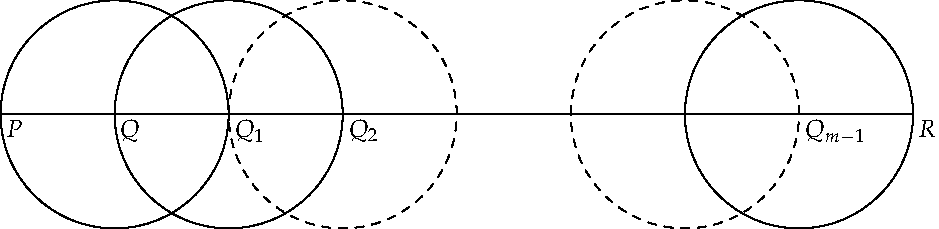
\includegraphics{const-int}
\end{center}

% \begin{cor}
% The set of integers $\Z$ is constructible: simply take $\{P,Q\}=\{0,1\}$ in the above and repeat with the roles of $P,Q$ swapped.
% \end{cor}

\begin{prop}\label{prop:const-bisect}
Let $P$ and $Q$ be distinct points. Then the perpendiculars to $\cl{PQ}$ through $P,Q$ and the midpoint of $\cl{PQ}$ are all constructible from $\{P,Q\}$.
\end{prop}

\begin{proof}
For the midpoint, draw circles centered at $P$ and $Q$ respectively, with radius $\nm{PQ}$. The intersection points $A,B$ may be joined, producing the bisector.\\
The perpendiculars through $P$ and $Q$ may be constructed similarly. For instance, first extend the segment $\cl{PQ}$ and draw a circle centered at $P$ with radius $\nm{PQ}$ to produce the point $R$. The perpendicular bisector of $\cl{RQ}$ is the desired perpendicular at\footnote{Of course we should check that the given construction does the job: if we're assuming a rigorous version of Euclidean geometry, this is easy. Recall that we're working within analytic geometry (indeed within $\C$), so this can be assumed.} $P$.
\end{proof}

\begin{center}
\animategraphics[timeline=const-perps.tln,controls]{0.75}{_const-perps}{0}{4}\qquad\qquad 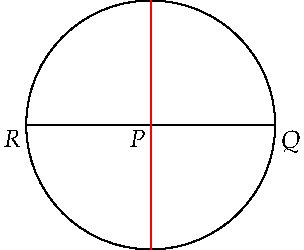
\includegraphics{const-perps2}
\end{center}

\begin{cor}
The set of Gaussian integers $\Z[i]=\{x+iy:x,y\in\Z\}$ is constructible.
\end{cor}

\begin{proof}
Proposition \ref{prop:const-int} applied to $\{P,Q\}=\{0,1\}$ constructs $\N_0$, now reverse the roles of $P,Q$ to construct the negative integers.\\
Given $x\in\Z$, Proposition \ref{prop:const-bisect} builds the perpendicular through $x$. Draw the circle radius 1 centered at $x$: one now obtains $x\pm i$. Proposition \ref{prop:const-int} now constructs the values $x\pm iy$ on this vertical line.
\end{proof}\pagebreak

\begin{prop}\label{prop:const-zbar}
Let $P,Q,R$ be non-collinear. Then the lines through $R$ parallel and perpendicular to $\overleftrightarrow{PQ}$ are both constructible from $\{P,Q,R\}$.
\end{prop}

\begin{proof}
Draw the circle with radius $\nm{PR}$ centered at $R$. Let $T$ be the other intersection of this circle with $\overleftrightarrow{PQ}$.
\begin{itemize}
  \item If $T=P$ so that there is only one intersection point, then $\overleftrightarrow{PQ}$ is tangent to the circle and thus the radius $\cl{PR}$ is perpendicular to $\overleftrightarrow{PQ}$.
  \item If $T\neq P$, then the perpendicular bisector of $\cl{PT}$ may be constructed. This passes through $R$ and is therefore the required line.
\end{itemize}
For the parallel line through $R$, construct the perpendicular to $\cl{PR}$ at $R$.
\end{proof}

\begin{cor}\label{prop:const-realimag}
$z=x+iy\in\C$ is constructible if and only if $x,y\in\R$ are constructible. In particular, $\cl z$ is constructible.
\end{cor}

\begin{proof}
If $y=0$ the result is trivial. Otherwise Proposition \ref{prop:const-zbar} constructs the parallel and perpendicular to $\R$ through $z$ and thus the intersection $x\in\R$ and $y\in i\R$. The circle centered at 0 with radius $iy$ intersects $\R$ at $y$. The converse follows from Proposition \ref{prop:const-bisect}. 
\end{proof}

\begin{prop}
Let $P$ and $Q$ be distinct points and let $r\in\Q$. Then any point $R\in\overleftrightarrow{PQ}$ for which  $\nm{PR}=r\nm{PQ}$ is constructible from $\{P,Q\}$.
\end{prop}

\begin{minipage}[t]{0.53\linewidth}\vspace{0pt}
\begin{proof}
\begin{itemize}\setlength{\itemsep}{2pt}
  \item Construct $m$ perpendicular to $\ell=\overleftrightarrow{PQ}$ through $P$.
  \item The circle center $P$, radius $\cl{PQ}$ constructs $S\in m$.
	\item Construct $n$ perpendicular to $m$ through 
$S$ and $T\in n$ such that $\nm{ST}=\nm{PQ}$.
	\item Given $q\in\N$, Proposition \ref{prop:const-int} defines $X$ such that $\nm{SX}=q\nm{ST}$.
	\item Define $Y=\overleftrightarrow{XQ}\cap m$.
	\item Finally define $Z =\overleftrightarrow{YT}\cap\ell$.
\end{itemize}\phantom{\qedhere}
\end{proof}
\end{minipage}
\begin{minipage}[t]{0.47\linewidth}\vspace{0pt}
\flushright\animategraphics[timeline=const-mult.tln,controls]{0.75}{_const-mult}{0}{5}
\end{minipage}\\
By similar triangles,
\[\frac{\nm{PZ}}{\nm{PQ}}=\frac{\nm{PZ}}{\nm{ST}} =\frac{\nm{PY}}{\nm{SY}} =\frac{\nm{PQ}}{\nm{SX}} =\frac 1q\]
Proposition \ref{prop:const-int} now allows us to construct $R$ such that $\nm{PR}=p\nm{PZ}=\frac pq\nm{PQ}$ for any $p\in\Z$.\hfill\qedsymbol

\begin{cor}
The rational numbers are constructible. Moreover, so is the extension field of rational complex numbers $\Q(i)=\{x+iy:x,y\in\Q\}$.
\end{cor}

\begin{cor}\label{cor:const-mult}
Suppose that $P,Q,A$ are constructible points on a line $\ell$ with $P$ distinct from $Q$ and $A$. Then the product $\nm{PQ}\nm{PA}$ and the quotient $\frac{\nm{PQ}}{\nm{PA}}$ are both constructible.
\end{cor}

\begin{proof}
Use the above picture: On the perpendicular to $\ell$ through $P$, construct $S$ and $Y$ such that $\nm{PY}=1$ and $\nm{PA}=\nm{YS}$. Then
\[\frac{\nm{SX}}{\nm{SY}} =\frac{\nm{PQ}}{\nm{PY}} \implies \nm{SX}=\nm{PQ}\nm{SY}=\nm{PQ}\nm{PA}\]
Similarly
\[\nm{PZ}=\frac{\nm{PZ}}{\nm{PY}} =\frac{\nm{ST}}{\nm{SY}} =\frac{\nm{PQ}}{\nm{PA}}\tag*{\qedhere}\]
\end{proof}

To complete the proof of Theorem \ref{thm:const-field} we put everything together:

% \begin{proof}[Proof of Theorem \ref{thm:const-field}]
% The constructible numbers are certainly a subset $\cC\subseteq\C$. We show that they are a subfield:
\begin{itemize}
  \item Addition/subtraction in $\R$:\quad Suppose that $x,y$ are constructible real numbers. Draw the circle centered at $x$ with radius $\nm y$. Its intersections with the real line are at $x\pm y$.
  \item Multiplication/division in $\R$:\quad If $x,y$ are positive constructible real numbers, Corollary \ref{cor:const-mult} takes care of things. Otherwise, apply the same construction to $\nm{x},\nm{y}$ and with suitable reflection to take care of any sign ambiguities.
  \item In $\C$: If $z=x+iy$ and $w=p+iq$ are constructible, then $z\pm w$, $zw$ and $\frac zw$ may all be expressed in terms of operations of real numbers. For instance, if $w\neq 0$,
  \[\frac zw=\frac{x+iy}{p+iq}=\frac{(xp+yq)+i(yp-xq)}{p^2+q^2}\]
  which is constructible since its real and imaginary parts are (Corollary \ref{prop:const-realimag}).
\end{itemize}
The constructible numbers are closed under the the field operations of $\C$: they are therefore a subfield.
We have moreover seen that all rational numbers are constructible: thus $\Q\subseteq\cC\subseteq\C$.
% \end{proof}


\subsubsection*{Square-roots and Angle-bisectors}

We've shown that all complex rationals $\Q(i)$ are constructible. The first obvious constructible irrationals are \emph{square-roots}. For instance, we can construct a square of side length 1, so we can also construct its hypotenuse of length $\sqrt 2$. It will transpire that sequences of square roots are essentially the \emph{only} additional numbers we can construct.\\

To start the discussion, we consider angles.

\begin{prop}
An angle with measure $\alpha$ is constructible if and only if $\cos\alpha\in\R$ is constructible.
\end{prop}

\begin{minipage}[t]{0.65\linewidth}\vspace{0pt}
\begin{proof}
If $\cos\alpha$ is constructible, intersect the perpendicular through $\cos\alpha$ with the unit circle to obtain the point $e^{i\alpha}=\cos\alpha+i\sin\alpha$. Joining this to 0 constructs $\alpha$.\\[5pt]
Conversely, given an angle $\alpha$ at $P$, draw the circle of radius 1 centered at $P$, thus producing two intersections $A,B$ with the rays defining $\alpha$. Drop the perpendicular from $B$ to $\ray{PA}$ to measure $\cos\alpha$.
\end{proof}
\end{minipage}\begin{minipage}[t]{0.35\linewidth}\vspace{0pt}
\flushright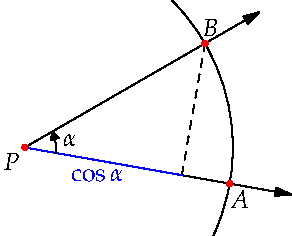
\includegraphics{const-angle}
\end{minipage}


\begin{prop}\label{prop:const-bisect2}
Let $\ell$ and $m$ be constructible lines intersecting at $P$. Then the line through $P$ bisecting an angle between $\ell$ and $m$ is constructible.
\end{prop}

\begin{proof}
Draw a circle of constructible radius centered at $P$. Let $A,B$ be intersections of the circle with each the lines $\ell,m$ respectively. The perpendicular bisector of $\cl{AB}$ (Propostion \ref{prop:const-bisect}) passes through $P$. SSS congruence forces this to be the angle bisector.
\end{proof}

\begin{cor}
If $\cos\alpha$ is constructible, then $\pm\cos\frac{\alpha}{2},\pm\sin\frac{ 
\alpha}{2}$ are also constructible.
\end{cor}

\begin{prop}
If $r\in\R^+$ is constructible, so is $\sqrt r$.
\end{prop}

A simpler proof is in the homework: here we continue the idea of bisecting angles.

\begin{proof}
For any integer $n$, the number $\frac{2r}{n^2}-1$ is also constructible. Choose $n$ large enough so that $-1<\frac{2r}{n^2}-1<1$. Put $\cos\alpha =\frac{2r}{n^2}-1$. Then, 
\[\cos\frac{\alpha}{2}=\sqrt{\frac{1+\cos\alpha}{2}}=\frac{\sqrt{r}}{n}\] 
is constructible and hence so is $\sqrt{r}$.
\end{proof}

\begin{cor}\label{cor:const-root}
For any $z\in\C$, the numbers $\sqrt z$ is constructible.
\end{cor}

The trick is to recall the form of a complex number in polar form:
\[z=re^{i\theta}\quad\text{where}\quad r=\nm z\quad\text{and}\quad \theta=\arg(z)\]
The square-roots is then $\sqrt z=\sqrt re^{i\theta/2}$. The upshot is that we are a constructible distance along a constructible angle bisector.



\subsubsection*{A complete description of the constructible numbers}

The remaining discussion may seem a little technical: you don't need to be familiar with field extensions to understand it, though it certainly makes things easier!
% \begin{itemize}
%   \item If we have a set $\F$ of constructible numbers, anything we can construct in one step using $\F$ must satisfy a degree one or two polynomial with coefficients in $\F$.
%   \item Any constructible number $z\in\cC$ satisfies a degree $2^n$ polynomial with coefficients in $\Q$.
% \end{itemize}

\begin{thm}
Suppose that a field $\F\subseteq\C$ is constructible from $\{0,1\}$ and closed under complex conjugation. Let $z\in\C$.
\begin{enumerate}
  \item If $z$ is constructible in one step from points in $\F$, then it is a zero of a linear or quadratic polynomial with coefficients in $\F$.
  \item If $z$ is a zero of a linear or quadratic polynomial with coefficients in $\F$, then $z$ is constructible in a finite number of steps from $\F$.
\end{enumerate}
% In the language of field extensions,
% \[\text{$z$ is constructible in one step from $\F\implies [\F(z):\F]=1$ or 2 $\implies$ every $w\in\F(z)$ constructible from $\F$}\].
\end{thm}

\begin{proof}
If a line joins two points $\sigma,\tau\in\F$, then it is easily seen to have equation
\[(\cl\tau-\cl\sigma)z-(\tau-\sigma)\cl z+\cl\sigma\tau-\sigma\cl\tau=\alpha z-\cl\alpha \cl z+\beta=0\]
with $\alpha,\beta\in\F$. Let $\delta,\eta,\zeta\in\F$: the circle centered at $\delta$ with radius $\nm{\eta-\zeta}$ has equation
\[(z-\delta)(\cl z-\cl\delta)=\nm\rho^2\]
where $\nm{\rho}^2=(\eta-\zeta)(\cl\eta-\cl\zeta)\in\F$.
We have three options for constructing a point $z$:
\begin{itemize}
  \item $z$ is the intersection of two lines. Eliminate $\cl z$ and solve for $z$ which lies in $\F$ (depends only on the coefficients and the field operations $+,-,\cdot,\div$).
	\item $z$ is an intersection of a line and a circle. Substitute the line equation in the circle to obtain a quadratic equation for $z$ with coefficients in $\F$.
	\item $z$ is the intersection of two circles. Given $(z-\delta)(\cl z-\cl\delta)=\nm\rho^2$ and $(z-\gamma)(\cl z-\cl\gamma)=\nm\sigma^2$, eliminate $\cl z$ to again obtain a quadratic equation for $z$ with coefficients in $\F$.
\end{itemize}
Conversely, if $z_0$ is a zero of a linear or quadratic polynomial $f$ with coefficients in $\F$, then we may compute $z_0$ from $\F$ using, at most, the quadratic formula. Since this only requires the field operations and computing a square-root, we see that $z_0$ is constructible from $\F$ (Corollary \ref{cor:const-root}).
\end{proof}

\paragraph{Example}

Describe a construction from $\Q$ of the roots of the polynomial $z^2+\frac 12z+\frac{11}{16}=0$.\\[5pt]
There are many, many ways to do this. Here is a construction using the intersection of two circles with rational radius centered at a rational point. We have $z_0,z_1=\frac 14(-1\pm\sqrt{10}i)$. Consider the picture, where $C$ is to be the center of a circle passing through $z_0=\frac 14(-1+\sqrt{10}i)$.
\begin{center}
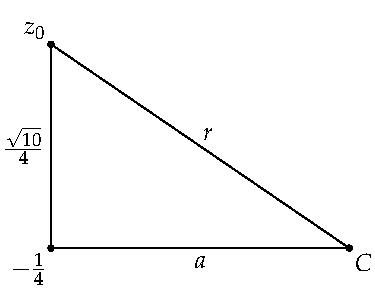
\includegraphics{const-example}\qquad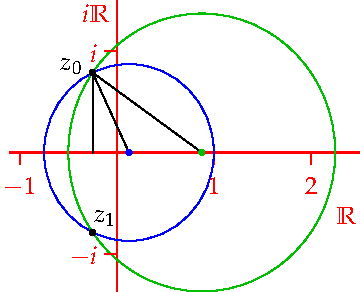
\includegraphics{const-example2}
\end{center}
If $C\in\Q$, we require $a$ and $r$ to be rational. By Pythagoras', we see that
\[r^2=a^2+\frac{10}{16}\implies (r-a)(r+a)=\frac 58\]
We can easily find many solutions $(a,r)\in\Q^2$ to this equation. For instance
\[\begin{cases}
r-a=\frac 14\\
r+a=\frac 52
\end{cases}\implies (a,r)=(\tfrac 98,\tfrac{11}8)\qquad\text{and}\qquad
\begin{cases}
r-a=\frac 12\\
r+a=\frac 54
\end{cases}\implies (a,r)=(\tfrac 38,\tfrac 78)\]
We therefore choose circles centered at $-\frac 14+a=\frac 18$ and $\frac 78$ with radii $\frac 78$ and $\frac{11}8$ respectively. Indeed one can check that
\[\begin{cases}
(z-\frac 18)(\cl z-\frac 18)=\left(\frac 78\right)^2\\
(z-\frac 78)(\cl z-\frac 78)=\left(\frac{11}8\right)^2
\end{cases}\implies z^2+\frac 12z+\frac{11}{16}=0\]
If complex numbers make this seem too difficult, observe that
\[\begin{cases}
(x-\frac 18)^2+y^2=\left(\frac 78\right)^2\\
(x-\frac 78)^2+y^2=\left(\frac{11}8\right)^2
\end{cases}\implies x=-\frac 14,\ y=\pm\frac{\sqrt{10}}4\]
\goodbreak

We make the following observations without proof (take a rings and fields class for details):
\begin{itemize}
  \item If $\F\subseteq\C$ is a field and $P\in\C$, then the \emph{extension field} $\F(P)$ is the collection of all complex numbers which may be produced from $\F$ and $P$ using only the field operations ($+,-,\cdot,\div$).
  \item $\F(P)$ is a vector space of degree $n$ over $\F$ if and only if the lowest-degree polynomial equation with coefficients in $\F$ satisfied by $P$ has degree $n$. We may write
  \[\F(P)=\{a_0+a_1P+\cdots+a_{n-1}P^{n-1}:a_i\in\F\}\]
  When the polynomial in question is \emph{monic} (leading term $x^n$), we call it the \emph{minimal polynomial of $P$}. The \emph{index} $[\F(P):\F]=n$ is the dimension of this vector space. 
\end{itemize}

\paragraph{Examples}

\begin{enumerate}
  \item The minimal polynomial of $P=i$ over $\Q$ is $x^2+1$. We can form the index-two  extension field $\Q(i)=\{q_0+q_1i:q_0,q_1\in\Q\}$.
  \item The minimal polynomial of $P=\sqrt[3]{2}$ over $\Q$ is cubic: $x^3-2$, whence the extension field has index $[\Q(\sqrt[3]{2}):\Q]=3$.
\end{enumerate}



\begin{cor}
\begin{enumerate}
  \item If $\F$ is a constructible field of finite index over $\Q$, then $[\F:\Q]=2^n$ for some $n\in\N$. In particular, there exist a tower of fields
  \[\Q=\F_0\le\F_1\le\cdots\le\F_n=\F\]
  such that $[\F_{k+1}:\F_k]=2$ for each $k$.
	\item If $z\in\C$ is constructible,\footnote{The field $\cC$ of constructible numbers is an \emph{infinite algebraic} field extension of $\Q$. Every element thus lies in some finite extension field $\F$ as in part 1.} then it has minimal polynomial over $\Q$ of degree $2^n$ for some $n\in\N$.
\end{enumerate}
\end{cor}


\subsubsection*{The impossible problems of antiquity}

The early Greek mathematicians took it almost as a point of faith that the solution to every problem could be constructed: all one had to do was to search hard enough and an explicit construction could be found. There were three problems, however, which were simple to state, yet for which no convincing constructions could be found. Mathematicians spent centuries searching for these. It wasn't until the modern advent of field theory that the non-existence of solutions to these problems could be proved.
% All you need to believe these proofs is the concept of an irreducible polynomial over $\Q$: this is a polynomial which cannot be factorized over the rationals; for the first two results, we could use, for instance, the rational roots theorem to show that the given cubic is irreducible. 

\begin{thm}
The following constructions are impossible with a ruler and compass:
\begin{enumerate}
  \item To duplicate a cube (draw a cube with double the volume of a 
given cube).
	\item To trisect a given angle.
	\item To square a circle\footnote{This expression has become a metaphor for attempting to do something impossible. You might hear it uttered by a politician to rubbish an opponents policy. Interestingly, the metaphor dates from a long time before the first proof of the impossibility, thus suggesting that belief predated proof!} (draw a square whose area equals that of a given circle). 
\end{enumerate}
\end{thm}

\begin{proof}
\begin{enumerate}
  \item If we could duplicate the cube, the ratio of the side lengths $\sqrt[3]{2}$ would have to be constructible. As observed above, the minimal polynomial of $\sqrt[3]{2}$ has degree three, whence $\sqrt[3]{2}$ is not constructible.
  \item We need a single counter-example. Consider the angle\footnote{This is itself constructible a the angle in an equilateral triangle.} $3\theta=\frac\pi 3$. If the angle $\theta=\frac\pi 9$ were constructible, so would be cosine $x=\cos\frac\pi 9$. The triple-angle formula yields a polynomial equation for $x$:
	\[\cos 3\theta=4\cos^3\theta-3\cos\theta\implies \frac 12=4x^3-3x\]
	It can be seen that this is the lowest degree polynomial satisfied by $x$. We have $[\Q(x):\Q]=3$ which is not a power of 2.
	\item In 1882, Ferdinand von Lindemann proved that $\pi$ (and consequently $\sqrt\pi$) is \emph{transcendental}: there are no polynomials $f$ with coefficients in $\Q$ for which $f(\pi)=0$. To square a circle of constructible radius $r$ would require construction of a square with side length $\sqrt\pi r$. Since $\sqrt\pi$ has no minimal polynomial, it is not constructible.\qedhere
\end{enumerate}
\end{proof}
